\documentclass[11pt]{article}
\usepackage[T1]{fontenc}
\usepackage[utf8]{inputenc}
\usepackage{lmodern,microtype,amsmath,amssymb,amsthm,mathtools}
\usepackage[a4paper,margin=28mm]{geometry}
\usepackage{xcolor,xurl,booktabs,enumitem,tikz}
\usetikzlibrary{arrows.meta,calc}
\usepackage[unicode,colorlinks=true,linkcolor=blue!45!black,
 citecolor=green!35!black,urlcolor=blue!55!black]{hyperref}
\setlength{\emergencystretch}{2em}
\numberwithin{equation}{section}
\newtheorem{theorem}{Theorem}[section]
\newtheorem{proposition}[theorem]{Proposition}
\newtheorem{lemma}[theorem]{Lemma}
\newtheorem{corollary}[theorem]{Corollary}
\theoremstyle{definition}\newtheorem{definition}[theorem]{Definition}
\theoremstyle{remark}\newtheorem{remark}[theorem]{Remark}
\newcommand{\Vol}{\operatorname{Vol}}
\newcommand{\Rea}{\operatorname{Re}}
\newcommand{\ii}{\mathrm i}
\newcommand{\C}{\mathrm C}
\newcommand{\Lft}{\mathrm L}
\newcommand{\Rgt}{\mathrm R}
\newcommand{\calQ}{\mathcal Q}
\title{Shared face estimates and triangular gluing for planar link diagrams}
\author{}\date{}
\begin{document}
\maketitle
\begin{abstract}
The exact polynomial of a marked planar link diagram uses one variable
for each face, shared by all its appearances. We give finite criteria
on these common variables that bound every noncentral part of the
invariant over the full real spectral cube. A weak, non-strict balance
condition at the complete circle packing suffices: a common power
change of the face weights gives a linear entropy gain and only a
quadratic cost. A second theorem preserves arbitrary unabridged
sector certificates under an oriented triangular gluing, retaining
the single coefficient target at the joining face. Both criteria
imply the volume limit for independently sufficiently long fixed
signed fillings, using numbered finite, analytic and geometric
companion theorems. An explicit seventeen-region certificate and its
iterated tetrahedral attachments give marked diagrams outside weak
balance. The proof includes the finite-cover logic and the rigorous
interval verification of this example.
\end{abstract}

\section{Common face weights and the volume statement}

A local estimate for a crossing box becomes useful only after its
variables have been identified with those of its neighbors. Choosing
a separate modulus for each occurrence of a face would generally
estimate a different coefficient. We keep this identification
throughout, both when changing the complete packing weights and when
joining two diagrams.

Our input \(D\) is a finite oriented simple triangulation of the sphere,
with at least four vertices, together with a perfect matching of its
cubic dual. The \(R\) matched pairs comprise \(2R\) triangles and
\(R+2\) vertices. At pair \(e\) write the cyclic quadrilateral as
\((x_e,b_e,y_e,c_e)\), with matching diagonal \(x_ey_e\).
Its polynomial arguments are ordered \((x_e,b_e,c_e,y_e)\).
Choose a nonmatching edge \(uv\). The two corresponding face variables
are \emph{protected}: \(L_u=L_v=0\). Let \(V\) be the set of the
\(R\) remaining, ordinary faces.

The inverse-cut construction of \cite[Section 2]{Geometry} gives an
augmented link in \(S^3\) with these exact labels. Each matched pair
records a crossing circle, its twice-punctured disk and its ordered
two-strand collar. Retain \(\epsilon_e\in\{0,1,-1\}\) half twists in
that collar. Filling its primitive slope \(\mu_e+p_e\lambda_e\)
inserts the crossing power
\begin{equation}\label{pc:powers}
                         n_e=\epsilon_e-2p_e .
\end{equation}
The local parity pairings and the outside connections are part of
the input. In every knot statement below, following them must give
one main component, with no additional closed main component.

Write \(Y_D\) for the complete augmented exterior. Its circle packing
has zero curvatures at \(u,v\) and positive curvatures \(w_f^*\) at
ordinary faces. The scale of all ordinary curvatures is immaterial.
We use the absolutely normalized triangle potential
\begin{equation}\label{pc:entropy}
\begin{aligned}
 \Lambda(t)&=-\int_0^t\log|2\sin s|\,ds,\\
 e(a)&=\frac{\Lambda(\pi a)+\Lambda(\pi/2-\pi a)}{\pi},
                  \qquad 0\le a\le\tfrac12.
\end{aligned}
\end{equation}
\begin{equation}\label{pc:Q}
 \calQ(w_1,w_2,w_3)
 =\max_{\substack{a_i\ge0,\ \sum_i a_i=1/2\\a_i=0\ \text{if }w_i=0}}
       \left\{\sum_i e(a_i)+\sum_{w_i>0}a_i\log w_i\right\}.
\end{equation}
At least one weight in each triangle is positive. In particular,
\(\calQ(0,0,B)=\frac12\log B\). No logarithm of a protected weight
is taken. At a positive ordinary vector \(L\), put
\begin{equation}\label{pc:rates}
\begin{aligned}
 X_e=A_{e,\C}&=\calQ(x_e,b_e,y_e)+\calQ(x_e,c_e,y_e),\\
 A_{e,\Lft}&=\max\{\log c_e,\calQ(x_e,b_e,y_e)+\tfrac12\log c_e\},
                                                   &&c_e>0,\\
 A_{e,\Rgt}&=\max\{\log b_e,\calQ(x_e,c_e,y_e)+\tfrac12\log b_e\},
                                                   &&b_e>0.
\end{aligned}
\end{equation}
Here a face label in a function denotes its weight in \(L\).
The three labels describe actual disjoint path sectors, defined in
Section~\ref{pc:finite}. Left is absent if \(c_e\) is protected;
right is absent if \(b_e\) is protected. Call the remaining set \(S_e\)
and set
\[
 \Sigma_D=\left(\prod_{e=1}^R S_e\right)\setminus\{\C^R\},\qquad
 \Phi_D=\frac{\Vol(Y_D)}{2\pi}.
\]
Thus \(\Sigma_D\) consists of all locally allowed noncentral strings.
It includes strings whose eventual shared coefficient happens to be zero.

For a nonempty set \(B\subseteq\Sigma_D\) define the common-weight cost
\begin{equation}\label{pc:branch-cost}
 G_{D,B}(L)=\max_{\omega\in B}\sum_e A_{e,\omega_e}(L)
                                  -\sum_{f\in V}\log L_f.
\end{equation}
For a single string we write \(G_{D,\omega}\).
Every occurrence of the same face in this expression uses the same
coordinate \(L_f\).

\begin{theorem}[Finite shared-face criterion]\label{pc:cover}
Let \(D\) be as above. Suppose a finite collection of nonempty sets
\(B\subseteq\Sigma_D\) covers \(\Sigma_D\), and each set has a fixed
positive ordinary vector \(L^B\), such that
\begin{equation}\label{pc:cover-gap}
 g=\min_B\{\Phi_D-G_{D,B}(L^B)\}>0.
\end{equation}
Then there is a threshold \(T_D\), depending on these fixed data,
such that every fixed integer vector \(\boldsymbol p\) with
\(\min_e|n_e|>T_D\), and with the stated knot pairing, gives a
hyperbolic knot \(K_D(\boldsymbol p)\) satisfying
\begin{equation}\label{pc:volume}
 \lim_{N\to\infty}\frac{2\pi}{N}
       \log|\langle K_D(\boldsymbol p)\rangle_N|
       =\Vol(S^3\setminus K_D(\boldsymbol p)).
\end{equation}
The invariant is the reduced zero-framed Kashaev invariant, with
unknot value one. The limit is over all integer levels, including
both parities and composite levels. The signs and relative sizes of
the fixed long powers are unrestricted. If \(\Sigma_D\) is empty,
no witnesses are required and the same conclusion holds.
\end{theorem}

The theorem concerns the unchanged recorded diagram. It imposes no
tree or separator condition, but it does require a strict common-weight
certificate. We prove two ways of obtaining one. Weak balance at the
complete packing permits equality in every local comparison
(Theorem~\ref{pc:weak-balance}). Protected triangular gluing preserves
any certificate of the stated kind (Theorem~\ref{pc:gluing}).
The explicit seed in Theorem~\ref{pc:seed} shows why the latter
hypothesis is more useful than restricting every input to weak balance.

Belted sums of augmented link complements have a substantial geometric
theory; see Morgan et al.~\cite{Belted}. Van der Veen~\cite{Whitehead}
proved the volume conjecture for Whitehead chains. We do not identify
our marked operation with all such constructions, or claim that its
unmarked knot types avoid other known presentations. The assertion here
is closure of shared source estimates with the original targets and
primitive fillings retained. No classification result from that
literature is used in the proof.

\section{The exact source and the imported foundations}\label{pc:finite}

This section specifies the finite object being bounded and the
numbered companion results used later. In particular, the central
asymptotic is not an assumption about the whole invariant.

For \(N\ge3\), set \(d=N-1\), \(\theta=\pi/N\), and
\[
 s_j=2\sin(j\theta),\qquad
 \chi_N(z)=2T_N(z/2)+2,\qquad T_N(\cos t)=\cos Nt.
\]
On \(1,z,\ldots,z^d\), define the banded polynomial operator
\[
 \mathsf C z^j=2\cos((2j+1)\theta)z^j
       -s_j^2(x+y)z^{j-1}-s_js_{j-1}xy\,z^{j-2}.
\]
Negative powers vanish. The finite Fourier theorem
\cite[Proposition 4.1]{Finite} identifies this operator, after the
specified specializations, transpose and gauge, with each physical
residue block of the two-strand Casimir. Its characteristic polynomial
is \(\chi_N\). Use the polynomial divided difference
\[
 V_N(\sigma;\mathsf C)=
       \frac{\chi_N(\sigma)-\chi_N(\mathsf C)}{\sigma-\mathsf C},
 \qquad
 H_V(x,b,c,y;\sigma)=
       \sum_{0\le i\le j\le d}V_N(\sigma;\mathsf C)_{ij}b^ic^{d-j}.
\]
Division here is polynomial division, including at repeated roots.
The face polynomial has total degree \(d\), and spectral degree at
most \(d\).

Expanding a triangular inverse before clearing its denominator gives
decreasing paths \(j\to i\) with steps of length one or two. The
monomial \(b^ic^{d-j}\) accompanies the outer step weights and every
unused spectral row. For \(h=\lfloor d/2\rfloor\), partition them by
\begin{equation}\label{pc:partition}
\begin{array}{c|c}
 \text{sector}&\text{condition}\\ \hline
 \C&i\le h,\quad d-j\le h\\
 \Lft&d-j>h\\
 \Rgt&i>h .
\end{array}
\end{equation}
Since \(i\le j\), two one-sided conditions cannot hold together.
This partition is exhaustive. At odd levels its central zero-step
path appears once, and a path skipping the central row keeps its
unused spectral factor. Denote the resulting polynomials by
\(H_{V,s}\). A protected overloaded middle kills the corresponding
one-sided polynomial exactly.

Take the single original coefficient
\begin{equation}\label{pc:source}
 S_{N,\omega}(\boldsymbol\sigma)=
 \left[\prod_{f\in V}L_f^d\right]
 \left.\prod_{e=1}^R
 H_{V,\omega_e}(L_{x_e},L_{b_e},L_{c_e},L_{y_e};\sigma_e)
                                      \right|_{L_u=L_v=0}.
\end{equation}
Write \(S_N=\sum_{\omega\in\prod S_e}S_{N,\omega}\),
\(C_N=S_{N,\C^R}\), and \(D_N=S_N-C_N\).
Each has degree at most \(d\) in each separate spectral variable.
Only the fixed number of factors is used here; the total spectral
degree need not be at most \(d\).

\begin{proposition}[Finite evaluation and its norm]\label{pc:finite-import}
For the original marked diagram and any integer powers \(n_e\),
its raw reduced ribbon contraction is
\begin{equation}\label{pc:finite-filling}
 Z_N(\boldsymbol n)=
       \left(\bigotimes_e\mathcal L_N^{n_e}\right)S_N,\qquad
 Z_{N,\C}=
       \left(\bigotimes_e\mathcal L_N^{n_e}\right)C_N.
\end{equation}
For every complex polynomial \(P\) of separate degrees at most \(d\),
\begin{equation}\label{pc:norm}
 \left|\left(\bigotimes_e\mathcal L_N^{n_e}\right)P\right|
       \le\prod_e(1+|n_e|/2)\,\|P\|_{[-2,2]^R}.
\end{equation}
The prescribed zero-framing and enhanced-component corrections have
modulus one. Thus they do not change the exponential rate of \(Z_N\).
\end{proposition}
\begin{proof}[Imported proof and its hypotheses]
The coefficient identity is \cite[Theorem 9.1 and Corollary 9.2]{Finite};
the invariant comparison is its Theorem 10.1. These statements retain
the actual cups and caps, unrestricted reduced mark, primitive face
lattice, and even-level affine coset. In particular there is no
extra factor \(N^R\) multiplying \eqref{pc:source}.
Theorem 1.1 of that paper gives the one-variable norm;
successive application gives \eqref{pc:norm}. Its functional uses
both values and first normals at repeated spectral roots, and the
value at the odd simple root. The separate-degree condition just
verified is exactly its hypothesis. Negative powers are included.
\end{proof}

\begin{proposition}[Uniform local envelopes]\label{pc:local-import}
For any fixed positive ordinary vector \(L\), with the protected
coordinates zero, and each locally allowed label \(s\),
\[
 \limsup_{N\to\infty}\frac1N
 \log\sup_{\substack{\sigma\in[-2,2]\\
                    |Z_f|=L_f\ (f\in V),\ Z_u=Z_v=0}}
 |H_{V,s}(Z_x,Z_b,Z_c,Z_y;\sigma)|
                  \le A_{e,s}(L).
\]
The supremum includes every face phase and every real spectrum, and
the limit superior includes both level parities.
\end{proposition}
\begin{proof}[Imported proof and its hypotheses]
This is \cite[Theorem 1.1]{Local}. The required \(x_e+y_e>0\)
holds: in a simple sphere the unique edge between \(u,v\) is the
nonmatching marked edge, and so it cannot also be the matching
diagonal. The theorem retains both unused products for the one-sided
sectors and the odd skipped-row term for the central sector.
No complete packing condition is required of \(L\).
\end{proof}

\begin{proposition}[Nonzero central contribution and its volume]
\label{pc:central-import}
The complete weights satisfy
\begin{equation}\label{pc:complete}
 P(q):=\sum_e X_e(e^q)-\sum_{f\in V}q_f,\qquad
 P(q^*)=\min P=\Phi_D,\quad \nabla P(q^*)=0,
                  \quad q_f^*=\log w_f^* .
\end{equation}
For independently sufficiently long fixed signed powers the original
central contraction is eventually nonzero and has logarithmic rate
\begin{equation}\label{pc:central-rate}
 \lim_{N\to\infty}\frac1N\log|Z_{N,\C}|=\Rea S_{\boldsymbol n},
 \qquad
 2\pi\Rea S_{\boldsymbol n}
   =\Vol(S^3\setminus K_D(\boldsymbol p)),
 \qquad
 \Rea S_{\boldsymbol n}\longrightarrow\Phi_D
\end{equation}
as all \(|n_e|\to\infty\), independently.
\end{proposition}
\begin{proof}[Imported proof and its hypotheses]
The complete packing, positive labeled cut and stationary action
\eqref{pc:complete} are supplied by \cite[Theorem 1.1, Proposition 2.1
and Section 3]{Geometry}. Convexity of \(\calQ\) makes that stationary
point a global minimum. The ordinary graph is connected, and the
ordinary difference rows generate the primitive common-scale
quotient. Each matched pair has a positive outer weight and at least
one nonmonomial triangle. These are the geometric hypotheses of
\cite[Theorem 1.1]{Source}; it proves the nonzero holomorphic shared
coefficient expansion and the full complementary spectral strip
bound for \(C_N\).

With its notation the expansion has unit
\(\varepsilon_N=(-1)^{dR}\), level power
\(\alpha=(3R+1)/2\), and coefficient
\((2\pi)^{-(R-1)/2}/\sqrt{\det H_N}\).
Theorem 1.1 of \cite{Oscillatory} evaluates the entire original
filling sum under exactly those two source hypotheses. Section 7
of \cite{Source} records the normalization: its second parity factor
is \((-1)^{(N+1)R}\), so their product is one. The actual leading
term is
\begin{equation}\label{pc:packet}
 \Gamma_N(-2\ii)^R\sqrt{2\pi}\,N^{R+1/2}
 \frac{\prod_e\sin(2\pi z_{N,e})}
 {\sqrt{\det H_N(z_N)}\sqrt{\det Q_N}}\,
                         e^{NS_{N,\boldsymbol n}},
\end{equation}
with relative error tending to zero, nonzero limiting coefficient
after these level and unit factors, and
\(S_{N,\boldsymbol n}\to S_{\boldsymbol n}\).
Here \(z_N\) is the unit-charge saddle, \(H_N\) the face Hessian,
\(Q_N\) the negative spectral Hessian, and
\(\Gamma_N=\exp(\pi\ii d^2\sum_e n_e/(4N))\).
The finite action stays inside the exponential.

Finally \cite[Theorem 1.1 and Corollary 8.1]{Geometry} identifies this
limiting action with the smooth filling of the original disk slopes.
The local potentials agree by their complete values and their
continued spectral derivatives, as calculated in
\cite[Lemma 5.1]{Local}. The geometric proof fixes the small
logarithms before multiplying by the large slopes, proves
\(U_e+p_eV_e=-2\pi\ii\), keeps the main cusp complete, and compares
volume on the same filled fundamental chain. These numbered results
give \eqref{pc:central-rate}; a formal critical point alone would not.
\end{proof}

\section{Finite certificates and the whole remainder}

\begin{definition}[Unabridged certificate]\label{pc:certificate}
An unabridged certificate for \(D\), with gap \(g>0\), assigns a
positive shared ordinary vector \(L^\omega\) to every
\(\omega\in\Sigma_D\), such that
\[
                     G_{D,\omega}(L^\omega)\le\Phi_D-g.
\]
Only the local protected-overloaded labels have been removed from
\(\Sigma_D\). In particular no string is omitted because of a
separate global vanishing or cancellation argument.
\end{definition}

A finite cover as in Theorem~\ref{pc:cover} gives this definition by
assigning each string to a cover member containing it. Conversely,
one witness per string is a finite cover. For a Cartesian branch
\(B=\prod_e S_{B,e}\subseteq\Sigma_D\), its cost is
\[
 G_{D,B}(L)=\sum_e\max_{s\in S_{B,e}}A_{e,s}(L)
                                  -\sum_{f\in V}\log L_f.
\]
For a non-Cartesian branch, the maximum in \eqref{pc:branch-cost}
must retain its correlations. Passing to the Cartesian hull is an
upper bound, not an equality in general. Choosing a branch of a
local maximum is also not the same as selecting an actual path sector.

\begin{lemma}[Homogeneity and full spectators]\label{pc:homogeneity}
For \(\lambda>0\), every local rate increases by \(\log\lambda\)
when all its positive weights are multiplied by \(\lambda\).
Consequently every \(G_{D,B}\) is unchanged by common rescaling.
Moreover, with protected logarithms omitted,
\begin{equation}\label{pc:spectators}
\begin{aligned}
 \max\{A_\C,A_\Lft,A_\Rgt\}&=\max\{X,\log b,\log c\}=:H,\\
 \max\{A_\C,A_\Lft\}&=\max\{X,\log c\}=:H_{\neg\Rgt}.
\end{aligned}
\end{equation}
\end{lemma}
\begin{proof}
Every supported simplex in \eqref{pc:Q} has total load \(1/2\),
so \(\calQ(\lambda w)=\calQ(w)+\frac12\log\lambda\).
There are \(R\) local rates and \(R\) ordinary targets, proving
the first assertion. Testing the simplex vertex at \(b\) gives
\(\calQ(x,b,y)\ge\frac12\log b\); similarly for \(c\).
Thus every mixed term in \eqref{pc:rates} is at most \(X\).
This proves both exact maximum identities.
\end{proof}

\begin{lemma}[Shared coefficient bound]\label{pc:remainder}
A certificate with gap \(g\) gives
\begin{equation}\label{pc:cube-gap}
 \limsup_{N\to\infty}\frac1N
          \log\|D_N\|_{[-2,2]^R}\le\Phi_D-g.
\end{equation}
\end{lemma}
\begin{proof}
For a string \(\omega\), apply the multivariate Cauchy coefficient
formula to \eqref{pc:source} on its one shared torus
\(|Z_f|=L_f^\omega\). Proposition~\ref{pc:local-import} gives
\[
 |S_{N,\omega}(\boldsymbol\sigma)|
 \le \prod_{f\in V}(L_f^\omega)^{-d}
       \prod_e\sup_{\text{same torus}}
                   |H_{V,\omega_e}(Z;\sigma_e)|.
\]
On dividing the logarithm by \(N\), the difference between \(d/N\)
and \(1\) contributes only
\(N^{-1}\sum_f\log L_f^\omega\). Hence the limit superior of the
uniform spectral rate is at most \(G_{D,\omega}(L^\omega)\).
There are finitely many strings and fixed witnesses, so all local
errors are simultaneous for sufficiently large \(N\). Finally
\(D_N=\sum_{\omega\in\Sigma_D}S_{N,\omega}\); the triangle
inequality costs only the fixed factor \(|\Sigma_D|\).
This proves \eqref{pc:cube-gap} through both parities. No infimum
over weights has been interchanged with a maximum over strings.
\end{proof}

\begin{proof}[Proof of Theorem~\ref{pc:cover}]
Use \eqref{pc:norm} on \(D_N\). The powers are fixed, so its prefactor
has zero exponential rate. Thus
\[
 \limsup_N N^{-1}\log|Z_N-Z_{N,\C}|\le\Phi_D-g.
\]
Increase the independent long-filling threshold until all conclusions
of Proposition~\ref{pc:central-import} hold and
\(\Rea S_{\boldsymbol n}>\Phi_D-g/4\). For these fixed powers,
\eqref{pc:cube-gap} implies an eventual upper rate
\(\Phi_D-3g/4\), after absorbing the fixed norm constant and the
finite local errors. The central limit gives an eventual lower
rate \(\Rea S_{\boldsymbol n}-g/8\). Their ratio therefore tends
to zero exponentially. In particular \(Z_N\ne0\) for all large \(N\),
and \(Z_N/Z_{N,\C}=1+O_{\boldsymbol n}(e^{-cN})\) for some \(c>0\).
The unit normalization in Proposition~\ref{pc:finite-import} and
the actual volume identity \eqref{pc:central-rate} give
\eqref{pc:volume}. If \(\Sigma_D\) is empty, the remainder is zero
and the same conclusion follows directly.
\end{proof}

\section{Weak balance and a quantitative defect criterion}

The complete packing is a convenient starting point for a common
weight vector. It is not necessary that the final Cauchy weights
describe another circle packing.

For an original triangle \(t\), let \(I_t\subseteq V\) be its
ordinary corners, and write
\[
 Q_t(q)=\calQ((e^{q_i})_{i\in I_t},0\text{ at protected corners}).
\]
The scalar function \(e\) in \eqref{pc:entropy} satisfies
\[
 e(0)=e(1/2)=0,\quad e'(a)=\log\cot(\pi a),\quad
 e''(a)=-\frac{2\pi}{\sin(2\pi a)}<0.
\]
These formulas include the absolute normalization:
\(\Lambda(\pi/2)=0\), obtained by reflection and the double-angle
identity for the integral of \(\log\sin\).
Thus \(e\) is positive in the interior.

\begin{lemma}[Triangle loads and curvature]\label{pc:triangle-calculus}
If \(|I_t|\ge2\), set \(w_i=e^{q_i}\) and
\[
 D_t^2=\sum_{\{i,j\}\subseteq I_t}w_iw_j,\qquad
             a_{ti}=\frac1\pi\arctan(w_i/D_t).
\]
These are the unique maximizing loads in \eqref{pc:Q}. They obey
\[
 \partial_i Q_t=a_{ti},\qquad
 E_t(q):=Q_t(q)-q\cdot\nabla Q_t(q)=\sum_i e(a_{ti})>0.
\]
For a singleton row, \(Q_t=q_i/2\) and \(E_t=0\). In either case
\begin{equation}\label{pc:hessian}
 h^{\mathsf T}\nabla^2Q_t(q)h
 =\sum_{\{i,j\}\subseteq I_t}\kappa_{ij}^t(h_i-h_j)^2,
 \qquad
 0<\kappa_{ij}^t=\frac{w_iw_j}{2\pi D_t(w_i+w_j)}
                                               \le\frac1{4\pi}.
\end{equation}
\end{lemma}
\begin{proof}
For two entries the two tangent ratios are reciprocal. For three,
\(D_t^2-w_iw_j=w_k(w_i+w_j)\) and the tangent addition formula
show that the displayed angles sum to \(\pi/2\).
Also \(e'(a_{ti})+q_i=\log D_t\). Strict concavity gives the
maximizer; its interior location follows from the infinite positive
endpoint derivative, so the entropy is strictly positive.
Differentiating the angles gives the off-diagonal entry
\(-\kappa_{ij}^t\); with three entries the cancellation is
\(D_t^2+w_i^2=(w_i+w_j)(w_i+w_k)\).
Logarithmic homogeneity gives zero Hessian row sums, proving
the quadratic form. Finally
\(D_t\ge\sqrt{w_iw_j}\) and \(w_i+w_j\ge2\sqrt{w_iw_j}\)
give its bound.
\end{proof}

From now on \(q=\log w^*\) is the fixed complete vector. Define
\begin{equation}\label{pc:energy}
 \mathcal E=\frac1{4\pi}
       \sum_t\sum_{\{i,j\}\subseteq I_t}(q_i-q_j)^2
   =\frac1{2\pi}\sum_{\substack{ij\text{ a white edge}\\i,j\in V}}
                                      (q_i-q_j)^2 .
\end{equation}
The equality counts the two triangles at each ordinary edge.
It is invariant under changing the common complete scale.
For \(0<t<1\) use the shared vector \(L_f(t)=e^{(1-t)q_f}\).
Taylor's formula, \eqref{pc:complete} and \eqref{pc:hessian} give
\begin{equation}\label{pc:cost}
 0\le P((1-t)q)-\Phi_D
   =\int_0^t(t-s)q^{\mathsf T}\nabla^2P((1-s)q)q\,ds
   \le\tfrac12t^2\mathcal E.
\end{equation}

There is a useful direct form of the entropy gain. The function
\(Q_t\) is convex, being a supremum of affine functions of \(q\).
Its supporting tangent at \(q\) gives, for \(0<\beta\le1\),
\begin{equation}\label{pc:tangent}
 Q_t(\beta q)\ge Q_t(q)+(\beta-1)q\cdot\nabla Q_t(q)
                =\beta Q_t(q)+(1-\beta)E_t(q).
\end{equation}
This also holds exactly for singleton rows. No concavity assertion
about a maximum of different local sectors is involved.

If there is no allowed one-sided label, then \(\Sigma_D\) is empty
and Theorem~\ref{pc:cover} already applies. For the rest of this
section suppose at least one such label survives.
For each allowed side \(s=\Lft,\Rgt\) at box \(e\), let \(z\)
be its overloaded middle (\(c_e\) for left, \(b_e\) for right),
and let \(t(e,s)\) be the triangle containing \(z\). Put
\begin{equation}\label{pc:defects}
 \epsilon_{e,s}=\max\{0,q_z-X_e(e^q)\},\qquad
                     h_{e,s}=E_{t(e,s)}(q).
\end{equation}
Every \(h_{e,s}>0\). Indeed \(z\) is ordinary and positive, while
at least one outer coordinate is ordinary because its matched edge
cannot be the protected nonmatching edge. Thus this triangle is
not a singleton.

\begin{lemma}[Loss for each side]\label{pc:side-loss}
For every allowed one-sided label and \(0<t<1\),
\begin{equation}\label{pc:loss}
 (X_e-A_{e,s})(L(t))
       \ge t h_{e,s}-(1-t)\epsilon_{e,s}.
\end{equation}
\end{lemma}
\begin{proof}
For left, writing \(Q_b=Q(x,b,y)\) and \(Q_c=Q(x,c,y)\),
\[
 X-A_\Lft=\min\{X-\log c,\ Q_c-\tfrac12\log c\}.
 \]
At \(q\), the first entry is at least \(-\epsilon_{e,\Lft}\).
The second is nonnegative, by the simplex vertex at \(c\).
Apply \eqref{pc:tangent} with \(\beta=1-t\). The first entry
gains \(t(E_b+E_c)\), at least \(t h_{e,\Lft}\), and the
second gains \(tE_c=t h_{e,\Lft}\). Both are bounded below
by the right side of \eqref{pc:loss}. Right is the same calculation
with \(b,c\) exchanged.
\end{proof}

\begin{theorem}[Weak balance and controlled defects]\label{pc:weak-balance}
Suppose for some \(0<t<1\)
\begin{equation}\label{pc:defect-criterion}
 \gamma(t)=
 \min_{(e,s)\text{ allowed}}
       \{t h_{e,s}-(1-t)\epsilon_{e,s}\}
                       -\tfrac12t^2\mathcal E>0.
\end{equation}
Then \(L(t)\) is an unabridged certificate with gap \(\gamma(t)\);
hence Theorem~\ref{pc:cover} applies. In particular it suffices that
the complete packing be \emph{weak-balanced}:
\begin{equation}\label{pc:weak}
 X_e(w^*)\ge\log w_b^*\quad(b\in V),\qquad
 X_e(w^*)\ge\log w_c^*\quad(c\in V)
\end{equation}
at every box, with equality allowed.
\end{theorem}
\begin{proof}
Let \(J(\omega)\) be the one-sided positions of a noncentral string.
Its cost at \(L(t)\) is exactly \(P((1-t)q)\) minus the sum of
the corresponding local losses. Equations \eqref{pc:cost} and
\eqref{pc:loss} give
\[
 G_{D,\omega}(L(t))\le
 \Phi_D+\tfrac12t^2\mathcal E-
       \sum_{(e,s)\in J(\omega)}
                 \{t h_{e,s}-(1-t)\epsilon_{e,s}\}.
\]
Condition \eqref{pc:defect-criterion} makes each summand positive,
and \(J(\omega)\) is nonempty. This proves the certificate.
Under \eqref{pc:weak}, all defects vanish. Let \(h_*=\min h_{e,s}>0\).
If \(\mathcal E>0\), choose
\[
 t_0=\min\{1/2,h_*/\mathcal E\};
 \quad\text{if }\mathcal E=0,\quad t_0=1/2.
\]
Then \(\gamma(t_0)\ge t_0h_*/2>0\). If there are no allowed
one-sided labels, the certificate is vacuous.
\end{proof}

The quantitative statement also allows positive balance defects:
with this \(t_0\), the sufficient condition
\(\max\epsilon_{e,s}<t_0h_*/2\) gives a gap at least
\(t_0h_*/2-\max\epsilon_{e,s}\).
All constants are computed on the original complete packing.
They are not claimed uniform over growing diagrams.

\begin{figure}[ht]
\centering
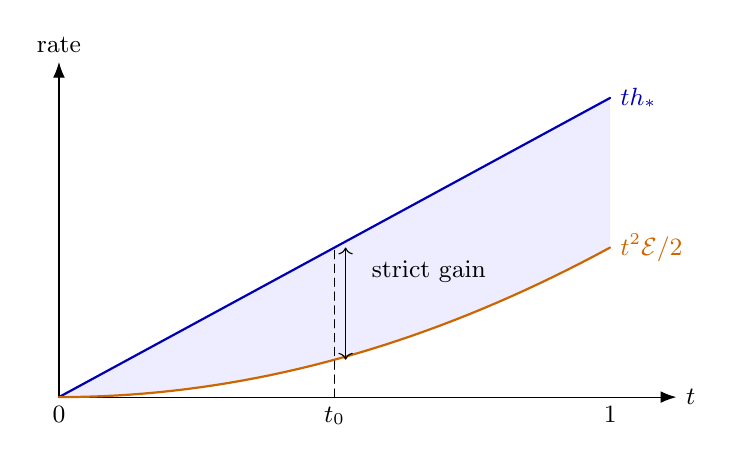
\begin{tikzpicture}[x=7cm,y=3.8cm,font=\small,
  line cap=round,line join=round]
 \fill[blue!7] (0,0)--plot[domain=0:1,samples=40](\x,\x)
        --plot[domain=1:0,samples=40](\x,{.5*\x*\x})--cycle;
 \draw[-{Latex[length=2mm]}] (0,0)--(1.12,0) node[right] {$t$};
 \draw[-{Latex[length=2mm]}] (0,0)--(0,1.12) node[above] {rate};
 \draw[blue!70!black,thick,domain=0:1,samples=2]
        plot(\x,\x) node[right] {$t h_*$};
 \draw[orange!80!black,thick,domain=0:1,samples=40]
        plot(\x,{.5*\x*\x}) node[right] {$t^2\mathcal E/2$};
 \draw[densely dashed] (.5,0)--(.5,.5);
 \draw[<->] (.52,.125)--(.52,.5);
 \node[anchor=west] at (.55,.42) {strict gain};
 \node[below] at (0,0) {$0$};
 \node[below] at (.5,0) {$t_0$};
 \node[below] at (1,0) {$1$};
\end{tikzpicture}

\caption{The common-weight change \(q\mapsto(1-t)q\). The lower bound
for one local loss is linear; the upper bound for the full action
cost is quadratic. The drawing uses \(h_*=\mathcal E=1\) only to
show their orders. In a diagram both constants are defined by its
shared ordinary face weights and original triangles.}
\label{pc:gain-figure}
\end{figure}

\section{Protected triangular gluing}\label{pc:joining}

We now permit different witnesses for different strings. This
flexibility makes a local gluing inequality survive the global
coefficient extraction.

Take two input spheres. Choose one triangle incident to each marked
edge and identify their boundary vertices as \(u,v,B\), where
\(u,v\) are protected and \(B\) is ordinary. Align their matched
sides and record the opposite orientations as
\begin{equation}\label{pc:old-pairs}
\begin{array}{c|c|c}
 &\text{removed oriented face}&\text{old polynomial quartet}\\ \hline
 D_1&(u,v,B)&(u,v,c,B)\\
 D_2&(u,B,v)&(u,a,v,B).
\end{array}
\end{equation}
If an entire input must be reflected to arrange this convention,
transport its cyclic orders, left/right labels and signed collars
with the reflection. The entropy bounds are unchanged.
Interior vertices from the two inputs are distinct.

Delete the two faces, identify their boundaries, and pair their old
partners \((u,a,B)\) and \((u,B,c)\). The new quartet is
\begin{equation}\label{pc:new-pair}
                              (u,a,c,B).
\end{equation}
Every other oriented face and matching pair is retained.
The punctured input spheres are disks; joining their boundaries
with opposite orientations gives an oriented sphere. There are no
new repeated vertices or edges apart from the identified boundary
ones, so the triangulation is simple. The new matching edge is
\(uB\), and the retained \(uv\) is nonmatching. Every triangle is
paired once. The counts are
\begin{equation}\label{pc:counts}
 R=R_1+R_2-1,\qquad |V_{\rm all}|=R+2,\quad
                         |F|=2R,\quad |E|=3R.
\end{equation}
The inverse cut therefore realizes an actual new augmented link
in \(S^3\), with its own primitive disks. This is an operation on
the recorded diagrams; it is not an asserted factorization of their
filled invariants.

\begin{figure}[htbp]
\centering
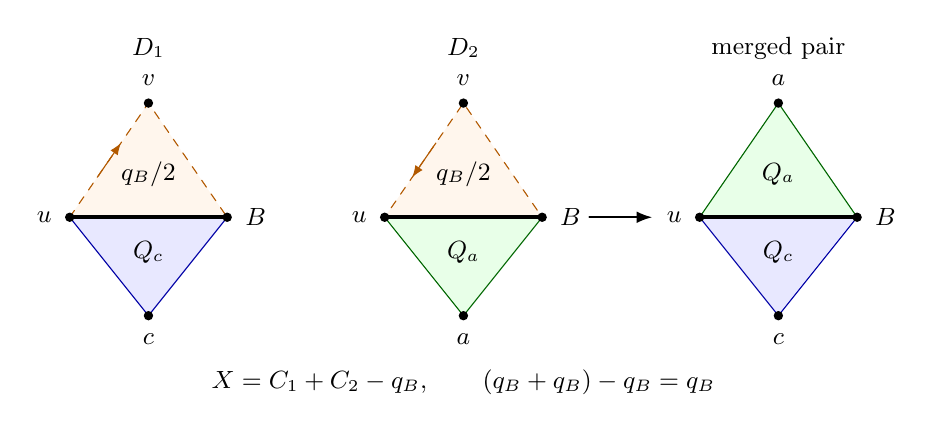
\begin{tikzpicture}[x=1cm,y=1cm,font=\small,line cap=round,line join=round,
 dot/.style={circle,fill=black,inner sep=1.2pt},
 removed/.style={draw=orange!70!black,dashed,fill=orange!7},
 piecea/.style={draw=green!40!black,fill=green!9},
 piecec/.style={draw=blue!65!black,fill=blue!9}]
 \begin{scope}
  \coordinate (u) at (0,0);\coordinate (B) at (2,0);
  \coordinate (v) at (1,1.45);\coordinate (c) at (1,-1.25);
  \path[removed] (u)--(v)--(B)--cycle;
  \draw[orange!70!black,-{Latex[length=1.5mm]}]
       ($(u)!.35!(v)$)--($(u)!.65!(v)$);
  \path[piecec] (u)--(B)--(c)--cycle;
  \draw[line width=1.6pt] (u)--(B);
  \foreach \p/\lab/\pos in {u/u/left,B/B/right,v/v/above,c/c/below}{
   \node[dot] at (\p) {};\node[\pos=3pt] at (\p) {$\lab$};}
  \node at (1,.55) {$q_B/2$};\node at (1,-.45) {$Q_c$};
  \node at (1,2.15) {$D_1$};
 \end{scope}
 \begin{scope}[xshift=4cm]
  \coordinate (u) at (0,0);\coordinate (B) at (2,0);
  \coordinate (v) at (1,1.45);\coordinate (a) at (1,-1.25);
  \path[removed] (u)--(B)--(v)--cycle;
  \draw[orange!70!black,-{Latex[length=1.5mm]}]
       ($(v)!.35!(u)$)--($(v)!.65!(u)$);
  \path[piecea] (u)--(a)--(B)--cycle;
  \draw[line width=1.6pt] (u)--(B);
  \foreach \p/\lab/\pos in {u/u/left,B/B/right,v/v/above,a/a/below}{
   \node[dot] at (\p) {};\node[\pos=3pt] at (\p) {$\lab$};}
  \node at (1,.55) {$q_B/2$};\node at (1,-.45) {$Q_a$};
  \node at (1,2.15) {$D_2$};
 \end{scope}
 \draw[-{Latex[length=2mm]},thick] (6.6,0)--(7.4,0);
 \begin{scope}[xshift=8cm]
  \coordinate (u) at (0,0);\coordinate (B) at (2,0);
  \coordinate (a) at (1,1.45);\coordinate (c) at (1,-1.25);
  \path[piecea] (u)--(a)--(B)--cycle;
  \path[piecec] (u)--(B)--(c)--cycle;
  \draw[line width=1.6pt] (u)--(B);
  \foreach \p/\lab/\pos in {u/u/left,B/B/right,a/a/above,c/c/below}{
   \node[dot] at (\p) {};\node[\pos=3pt] at (\p) {$\lab$};}
  \node at (1,.55) {$Q_a$};\node at (1,-.45) {$Q_c$};
  \node at (1,2.15) {merged pair};
 \end{scope}
 \node at (5,-2.1) {$X=C_1+C_2-q_B,\qquad
             (q_B+q_B)-q_B=q_B$};
\end{tikzpicture}

\caption{Only the shaded dashed faces are removed. Their boundaries
are identified with opposite orientations; \(u,v\) remain protected
and \(B\) becomes one ordinary face with one coefficient target.
The thick edge \(uB\) now matches the retained triangles. The vertex
\(v\), absent from this new pair, remains elsewhere in the sphere.
Writing \(q_B=\log B\), the removed triangle rates total \(q_B\).
This exactly compensates for counting the \(B\)-target once rather
than twice. The figure records the oriented triangles and their matching.}
\label{pc:gluing-figure}
\end{figure}

\begin{lemma}[The common complete action]\label{pc:action-sum}
When the two weight vectors agree at \(B\),
\begin{equation}\label{pc:action-add}
                   P_{\rm new}(q_1,q_2)=P_1(q_1)+P_2(q_2).
\end{equation}
Consequently \(\Phi_{\rm new}=\Phi_1+\Phi_2\). The complete
weights on each piece are its old weights up to a common rescaling.
\end{lemma}
\begin{proof}
Put \(Q_a=\calQ(0,a,B)\), \(Q_c=\calQ(0,c,B)\) and \(q_B=\log B\).
The two old complete rates and the merged rate are
\[
 C_1=\tfrac12q_B+Q_c,\qquad
 C_2=Q_a+\tfrac12q_B,\qquad X=Q_a+Q_c=C_1+C_2-q_B.
\]
Every other triangle term is unchanged. The two old target sums
count \(q_B\) twice and the new one once, proving
\eqref{pc:action-add}. Normalize the two complete minima by \(B=1\);
they then combine into a global minimum. Conversely the right
side is always at least the sum of its two minima. The marked
packing's uniqueness up to scale, supplied by \cite[Section 3]{Geometry},
identifies these complete weights.
\end{proof}

\begin{lemma}[All three merged sectors]\label{pc:merge}
The new sector has the following locally allowed input strings:
\begin{equation}\label{pc:merge-table}
\begin{array}{c|c|c}
 \text{new label}&\text{input labels}&\text{comparison}\\ \hline
 \C&(\C,\C)&X=C_1+C_2-q_B\\
 \Lft&(\Lft,\C)&A_\Lft\le L_1+C_2-q_B\\
 \Rgt&(\C,\Rgt)&A_\Rgt\le C_1+R_2-q_B.
\end{array}
\end{equation}
Here \(L_1\) and \(R_2\) are the old first-left and second-right
rates in their original frames.
\end{lemma}
\begin{proof}
Only left survives at the first old box and only right at the
second. Their rates are
\[
 L_1=\max\{q_c,\tfrac12q_B+\tfrac12q_c\},\qquad
 R_2=\max\{q_a,\tfrac12q_B+\tfrac12q_a\}.
\]
The simplex vertices at \(B\) give \(Q_a,Q_c\ge q_B/2\).
Therefore
\[
 L_1+C_2-q_B
 =\max\{q_c+Q_a-\tfrac12q_B,Q_a+\tfrac12q_c\}
 \ge\max\{q_c,Q_a+\tfrac12q_c\}=A_\Lft .
\]
Exchange \(a,c\) for the right inequality. Neither calculation
requires \(q_B\) to be positive. Both branches of the one-sided
maximum have been retained.
\end{proof}

\begin{theorem}[Closure of unabridged certificates]\label{pc:gluing}
If \(D_1,D_2\) have certificates in the sense of
Definition~\ref{pc:certificate}, with gaps \(g_1,g_2>0\), their
protected triangular gluing has one with gap at least
\(\min(g_1,g_2)\). Any fixed finite iteration satisfies
\begin{equation}\label{pc:iteration}
 R=\sum_jR_j-(k-1),\qquad
 \Phi=\sum_j\Phi_j,\qquad g\ge\min_jg_j.
\end{equation}
For every knot-producing parity pattern of the assembled diagram,
its independently sufficiently long fixed signed fillings satisfy
\eqref{pc:volume}.
\end{theorem}
\begin{proof}
Given any noncentral output string, use \eqref{pc:merge-table} at
the merged box and retain every other label on its original piece.
This yields locally allowed strings \(\omega_1,\omega_2\).
At least one is noncentral. The exact target cancellation gives
\[
 G_{{\rm new},\omega}(q_1,q_2)
                   \le G_{1,\omega_1}(q_1)+G_{2,\omega_2}(q_2)
 \quad\text{when }(q_1)_B=(q_2)_B.
\]
For a noncentral input choose its certificate vector. For a central
input choose its complete minimum. Rescale each whole vector to
\(B=1\) using Lemma~\ref{pc:homogeneity}. They now agree on all
shared variables: the protected zeros and this single ordinary
weight. Their costs give the claimed gap, using
Lemma~\ref{pc:action-sum}.

This reasoning uses every locally allowed induced string, whether
or not that string's old final coefficient vanishes. It would not
justify reusing a certificate that discarded such strings.
Repeated gluing preserves the simple sphere and the nonmatching
mark. At a later step rescale the entire previously assembled
vector, not its already identified faces independently.
Induction gives \eqref{pc:iteration}, and
Theorem~\ref{pc:cover} supplies the volume conclusion.
\end{proof}

A knot parity is always available, although the theorem also permits
any other parity passing the original component test. In the
untwisted diagram the physical strands are projection circles.
Make a graph with these circles as vertices and a box as an edge
joining the two circles meeting its disk; loops are allowed.
It is connected because the original four-valent projection is
connected. Choose a spanning tree and make exactly its boxes odd.
At each step the odd reconnection joins two distinct current
circles, so it merges them without producing an extra component.
Induction leaves one circle. Either odd sign has this pairing.
This does not claim that arbitrary old knot parities remain knots
after the gluing.

If both inputs are weak-balanced, the output is also weak-balanced.
At complete weights the unmerged comparisons are unchanged, while
\[
 X=Q_a+Q_c\ge C_1\ge q_c,\qquad
 X\ge C_2\ge q_a.
\]
The first inequalities use \(Q_a,Q_c\ge q_B/2\).
The more general certificate theorem is useful because its inputs
need not satisfy weak balance, as the next example shows.

\section{A certified seed outside weak balance}\label{pc:example}

We specify the finite example by its actual ordered quartet list,
so the argument does not require a diagram compiler to define the
source. Let the vertices be \(0,\ldots,18\), the protected edge be
\(\{0,16\}\), and take the following polynomial-order quartets:
\begin{equation}\label{pc:seed-quartets}
\begin{array}{c|c@{\qquad}c|c}
e&(x,b,c,y)&e&(x,b,c,y)\\ \hline
0&(1,0,4,2)&9&(10,8,13,0)\\
1&(2,0,5,3)&10&(11,9,14,12)\\
2&(0,1,6,4)&11&(12,10,15,13)\\
3&(4,2,7,5)&12&(0,11,16,14)\\
4&(5,3,8,0)&13&(14,12,17,15)\\
5&(6,4,9,7)&14&(15,13,18,0)\\
6&(7,5,10,8)&15&(16,14,0,17)\\
7&(0,6,11,9)&16&(17,15,0,18)\\
8&(9,7,12,10)&&
\end{array}
\end{equation}
Each row means the oriented faces \((x,b,y)\), \((x,y,c)\),
paired along \(xy\). The list gives 34 distinct faces and 51 edges;
every edge occurs twice with opposite directions. Each vertex link
is one cycle, the face adjacency graph is connected, and
\(19-51+34=2\). Thus it is an oriented simple sphere.
Its 17 matching edges are distinct and pair exactly the listed
faces; \(\{0,16\}\) is nonmatching. These finite combinatorial
assertions can be checked directly from the table by the procedure
in Section~\ref{pc:reproduce}.

\begin{theorem}[The seed and its attachments]\label{pc:seed}
The marked sphere \eqref{pc:seed-quartets} has an unabridged
forty-branch certificate with gap greater than \(1/25\).
Its complete packing fails weak balance at at least one of
the boxes
\[
                              J=\{2,4,7,12\}.
\]
For every fixed \(r\ge0\), it admits \(r\) successive tetrahedral
attachments that retain those boxes and yield an unabridged
certificate on \(17+r\) regions, still outside weak balance at the
retained mark. All knot-producing long fixed signed fillings of
these recorded diagrams satisfy \eqref{pc:volume}.
\end{theorem}

\subsection{The finite cover}
The positive rational data used below are the two committed
certificates \cite{CoverData,AnchorData}. We describe every kind
of entry and the inequalities they certify, including their
rigorous evaluation. The saved rational numbers are witnesses;
no numerical minimizer is an input to the proof.

There are two kinds of branches. For each nonempty subset of \(J\),
require right at exactly those positions of \(J\), allow central
or left at the other positions of \(J\), and all locally allowed
labels elsewhere. These are 15 branches. If no position of \(J\)
is right, choose any surviving one-sided label as an anchor, allow
central or left at the other positions of \(J\), and all labels
elsewhere. There are 25 such anchors. They cover every locally
allowed noncentral string: either its right subset in \(J\) is
nonempty, or it has a one-sided anchor in the second case.
No branch contains the all-central string. Overlap causes no
problem.

The file \cite{CoverData} stores one positive rational vector for
each branch, with the protected zeros retained. Its tags have the
following exact meanings:
\[
 H=\max\{X,q_b,q_c\},\qquad
 H_{\neg\Rgt}=\max\{X,q_c\},\qquad A_\Lft,\quad A_\Rgt .
\]
These are \eqref{pc:spectators}, not a replacement of a genuine
sector by an invented label. Undefined protected logarithms are
omitted.

The same file gives 83 nonnegative rational corner loads
\(\alpha_{ti}\), one for each supported triangle corner, with
\[
 \sum_{i\in I_t}\alpha_{ti}=\tfrac12,\qquad
                \sum_{t\ni f}\alpha_{tf}=1\quad(f\in V).
\]
Their entropy \(E_{\rm low}=\sum_{t,i}e(\alpha_{ti})\) is a
lower bound for \(\Phi_{17}\): test these loads in every
\(\calQ\) and cancel the ordinary target logarithms. This is
weak duality at every vector, followed by the minimum in
\eqref{pc:complete}.

The interval calculation detailed below proves
\begin{equation}\label{pc:seed-cover-values}
 E_{\rm low}>19.90751095350,\qquad
       \max_B G_{D,B}(L^B)<19.85303956990.
\end{equation}
Their difference exceeds \(0.05447>1/25\). This proves the
certificate assertion, including strings that might have zero
shared coefficient.

\subsection{Locating the failure of weak balance}
The second rational file \cite{AnchorData} gives a weak-duality
lower bound for the smaller comparison
\begin{equation}\label{pc:restricted}
 \widetilde G(q)=A_{12,\Rgt}(q)+
       \sum_{e\in\{2,4,7\}}H_e(q)+
       \sum_{e\notin J}X_e(q)-\sum_{f\in V}q_f.
\end{equation}
At spectator \(e\in\{2,4,7\}\), choose a rational mass
\(0<\lambda_e\le1\) for its two complete triangle rows and mass
\(1-\lambda_e\) on the pure \(b_e\)-coordinate. Each weighted
triangle row has loads \(\alpha_{ti}\ge0\) summing to
\(\lambda_e/2\), and entropy
\(\lambda_e\sum_i e(\alpha_{ti}/\lambda_e)\).
At the other non-anchor boxes \(\lambda_e=1\).
At anchor 12 the quartet is \((0,11,16,14)\), so
\[
 A_{12,\Rgt}=\max\{q_{11},(q_{11}+q_{14})/2\}.
\]
Choose loads \(1-\beta,\beta\) on faces \(11,14\), respectively,
with rational \(0\le\beta\le1/2\); their entropy is zero.
The file contains 84 rational variables in these weighted rows,
masses and anchor allocation. Every ordinary face load, including
the pure-middle and anchor loads, is exactly one.

The inequalities
\[
 \max\{X,q_b\}\ge\lambda X+(1-\lambda)q_b,\qquad
 A_{12,\Rgt}\ge(1-\beta)q_{11}+\beta q_{14}
\]
and the triangle variational formula show
\(\widetilde G(q)\ge E_{\rm flow}\) for every \(q\);
all logarithmic terms cancel. A separate positive rational vector
\(L^{\rm up}\) gives \(\Phi_{17}\le P(\log L^{\rm up})\).
Rigorous evaluation gives
\begin{equation}\label{pc:seed-obstruction-values}
 E_{\rm flow}>19.95975965735,\qquad
 P(\log L^{\rm up})<19.92324700353.
\end{equation}
It follows that \(\widetilde G(q)>\Phi_{17}+1/40\) for all \(q\).
If all four boxes of \(J\) were weak-balanced at the complete
vector, then \(H_e=X_e\) at \(2,4,7\), and
\(A_{12,\Rgt}\le X_{12}\) by the simplex inequality.
This would give \(\widetilde G(q^*)\le P(q^*)=\Phi_{17}\),
a contradiction.

This comparison does not assert that a fixed genuine sector has
rate exceeding volume. The three spectator mixtures are atoms of
the upper function \(H\). They serve here only to locate a failure
of weak balance in the recorded diagram.

\subsection{Reproducible exact and interval verification}\label{pc:reproduce}
The certificate files contain the quartet list, protected and ordinary
vertices, rational numbers as integer numerator--denominator pairs,
and the row and branch indices just described. The verifier first
checks these finite lists and all row and face sums with rational
arithmetic. For the topology it counts both oriented occurrences
of every edge, traces every vertex link, checks connected face
adjacency and Euler characteristic two, and verifies that each
matching edge pairs its two declared faces. These are complete
finite checks of this particular table, not samples of an
infinite family.

For a positive supported triangle, its potential is evaluated by
the formula proved in Lemma~\ref{pc:triangle-calculus}:
\[
 Q_t=\frac1\pi\sum_{i\in I_t}
 \left\{\Lambda(\vartheta_i)+
        \Lambda(\pi/2-\vartheta_i)+\vartheta_i\log w_i\right\},
 \quad
 \vartheta_i=\arctan\frac{w_i}{\sqrt{\sum_{i<j}w_iw_j}}.
\]
Singletons are half logarithms. All elementary operations use
outward ball arithmetic at 192 bits \cite{Arb}. For the only
infinite series, the absolutely convergent Fourier formula is
\begin{equation}\label{pc:lobachevsky-check}
 \Lambda(t)=\sum_{k=1}^{M}\frac{\sin(2kt)}{2k^2}+\mathcal R_M(t),
                       \qquad |\mathcal R_M(t)|\le\frac1{2M}.
\end{equation}
Indeed integrate the Abel-regularized Fourier series for
\(-\log|2\sin t|\), then pass to the uniformly convergent
integrated series. The tail is bounded by
\(\frac12\sum_{k>M}k^{-2}\le1/(2M)\).
Values \(e(0)=e(1/2)=0\) are inserted exactly.
Use \(M=2048\) in \eqref{pc:seed-cover-values} and \(M=8192\)
in \eqref{pc:seed-obstruction-values}. For a maximum of interval
enclosures, the lower bound is the maximum of their lower
endpoints and the upper bound is the maximum of their upper
endpoints. This bounds every branch including ties.

The command
\begin{verbatim}
python3 papers/planar-certificates/check.py --output /tmp/planar-check
\end{verbatim}
replays the two existing exact verifiers, checks the displayed
quartet table and orientations, and records all input hashes.
It requires Python with \texttt{python-flint} and NumPy. The two fixed
certificate SHA256 values are
\begin{quote}\small
\nolinkurl{54f6087e25e9e6c48e123ea61497cab2a2bb2eb3e4d92a2eb3f9b6e76452eadb}\\
\nolinkurl{8e9ca9b9baf9383449a54840a4204ac4008b20cd9a56684ffc9a0a45c65bba27}.
\end{quote}
Together with the explicit tail in \eqref{pc:lobachevsky-check},
these checks prove the finite inequalities used above. The
asymptotic and geometric conclusions are the written implications
of the preceding sections, not extrapolations from finite levels.

\subsection{Arbitrarily many attachments}
The marked-edge triangles of the seed are at boxes 12 and 15.
Use the latter's output face:
\[
              (x,b,c,y)_{15}=(16,14,0,17),\qquad (16,17,0).
\]
This is the second input of \eqref{pc:old-pairs}, with
\((u,v,B,a)=(16,0,17,14)\). Thus no box in \(J\) is changed.

For the other input take a tetrahedral sphere with oriented faces
\[
 (u,v,B),\quad(u,B,C),\quad(B,v,C),\quad(v,u,C),
\]
matching \(uB,vC\), and protected edge \(uv\).
Its quartets are \((u,v,C,B)\) and \((v,u,B,C)\).
At \(B=C=1\), each ordinary face receives load \(1/2\) from
one singleton and \(1/4\) from each of the two nonsingleton
triangles. It is therefore the complete stationary vector.
Each complete box rate is \(2e(1/4)>0\), whereas the positive
middle logarithm is zero. It is strictly balanced and has a
certificate by Theorem~\ref{pc:weak-balance}.

Continue on the newly added side of the retained marked edge,
using fresh vertices at each attachment. The original boxes of
\(J\) remain unchanged. Lemma~\ref{pc:action-sum} preserves their
complete weights up to a common scale, and
\(X_e-q_b,\ X_e-q_c\) are invariant under that scale. The original
failure of weak balance therefore persists. For \(r\) attachments,
\[
                 R_r=17+r,\qquad
                 \Phi_r=\Phi_{17}+4r\,e(1/4).
\]
Theorem~\ref{pc:gluing} provides the unabridged certificate and
Theorem~\ref{pc:cover} the knot volume limit. This proves
Theorem~\ref{pc:seed}. The fixed diagram and its parity pattern
are chosen before the independent long fillings and before \(N\).

\section{Scope of the criteria}

The two sufficient conditions have different uses. Weak balance
requires only the original complete packing and supplies one
common vector for all strings. Triangular gluing preserves the
more flexible assignment of a vector to each genuine string.
The seed gives an explicit strict distinction at a fixed mark;
it does not exclude another mark or another presentation of the
same knot from satisfying weak balance.

The gluing proof does not apply to a bound known only after
cancellation of the entire source, nor to a bound with some
spectral parameters fixed at their endpoints. Such bounds need
not supply the input vectors in \eqref{pc:merge-table}. Likewise,
discarding an input string because its coefficient vanishes
globally would require a separate support-transfer proof.
The unabridged definition avoids that unproved step.

No certificate is asserted for every simple matched sphere.
No threshold is uniform over a growing number of pieces or over
powers varying with the level. The full volume conclusions proved
here use the original spectral functional and primitive fillings
of each output diagram. They neither replace the invariant by a
positive model nor infer a volume from an unmarked critical point.

\begin{thebibliography}{12}
\bibitem{Finite}\emph{Finite spectral evaluation and uniform filling bounds}.
\url{https://sashakolpakov.github.io/murakamis_dream/papers/filling-bounds.pdf}.
\bibitem{Local}\emph{Uniform spectral bounds for local Casimir sources}.
\url{https://sashakolpakov.github.io/murakamis_dream/papers/local-coefficients.pdf}.
\bibitem{Source}\emph{Holomorphic asymptotics of central shared face coefficients}.
\url{https://sashakolpakov.github.io/murakamis_dream/papers/source-asymptotics.pdf}.
\bibitem{Oscillatory}\emph{Oscillatory filling sums with independently long twists}.
\url{https://sashakolpakov.github.io/murakamis_dream/papers/oscillatory-fillings.pdf}.
\bibitem{Geometry}\emph{Circle patterns and primitive fillings of augmented links}.
\url{https://sashakolpakov.github.io/murakamis_dream/papers/marked-fillings.pdf}.
\bibitem{CoverData}\emph{Rational shared-radius witnesses for the seventeen-region source}.
\href{https://github.com/sashakolpakov/murakamis_dream/blob/main/experiments/actual_sector_cover_certificate.json}{Certificate};
\href{https://github.com/sashakolpakov/murakamis_dream/blob/main/experiments/audit_actual_sector_cover.py}{exact verifier}.
\bibitem{AnchorData}\emph{Rational dual flow for the restricted anchored comparison}.
\href{https://github.com/sashakolpakov/murakamis_dream/blob/main/experiments/actual_shared_radius_anchor_obstruction_certificate.json}{Certificate};
\href{https://github.com/sashakolpakov/murakamis_dream/blob/main/experiments/audit_actual_shared_radius_anchor_obstruction.py}{exact verifier}.
\bibitem{Belted} P. Morgan, B. Ransom, D. Spyropoulos, C. Ziegler and R. Trapp,
\emph{Belted sum decompositions of fully augmented links}, 2023.
\url{https://arxiv.org/abs/2311.13540}.
\bibitem{Whitehead} R. van der Veen,
\emph{Proof of the volume conjecture for Whitehead chains},
Acta Math. Vietnamica 33 (2008), 421--431.
\url{https://arxiv.org/abs/math/0611181}.
\bibitem{Arb} F. Johansson,
\emph{Arb: Efficient arbitrary-precision midpoint-radius interval arithmetic},
2016. \url{https://arxiv.org/abs/1611.02831}.
\end{thebibliography}
\end{document}
